\lecture{3}{3. Februar 2025}{Crystalline solids}

\exercise{3.2}
If the atomic radius of lead is \qty{0,175}{nm}, calculate the volume of its unit cell in cubic meters.
\bigbreak
Lead has an FCC structure meaning that the (\textit{cubic}) unit cell has a side length of $a = 2R \sqrt{2}$, where $R$ is the atomic radius. Thus we get
\[ 
V_c = a^3 = \left( 2\sqrt{2} \cdot \qty{0,175}{nm}  \right)^3 = \qty{1,213e-28}{m^3} 
.\]


\exercise{3.5}
Strontium (Sr) has an FCC crystal structure, an atomic radius of \qty{0,215}{nm} and an atomic weight of \qty{87,62}{g/mol}. Calculate the theoretical density for Sr.
\bigbreak
We start by calculating the volume of the unit cell $V_c$ as above.
\[ 
V_c = \left( 2 \sqrt{2} \cdot \qty{0,215}{nm}  \right)^3 = \qty{2,249e-28}{m^3} 
.\]
We Should also note that for FCC the amount of atoms in the UC is 4. We can now calculate the theoretical density of strontium with the general formula
\[ 
\rho = \frac{nA}{V_c N_a}
.\]
Where $n$ is the amount of atoms in the UC, $A$ is the atomic weight, $V_c$ is the volume of the UC and $N_a$ is Avogadro's constant. By substituting values we get
\[ 
\rho_{\mathrm{Sr}} = \frac{4 \cdot \qty{87,62}{\frac{g}{mol}}}{N_a \cdot \qty{2,249e-28}{m^3}} = \qty{2,587}{\frac{g}{mol}} 
.\]


\exercise{3.13}
List the point indices for all atoms that are associated with the FCC unit cell (\textbf{\autoref{fig:e3_1}}).
\begin{figure} [ht]
  \centering
  \caption{}
  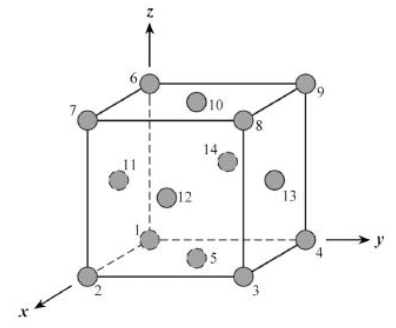
\includegraphics[width=0.5\linewidth]{../figures/e3_1.png}
  \label{fig:e3_1}
\end{figure}
\bigbreak
The point indices for the points in order are
\begin{enumerate}
  \item 000
  \item 100
  \item 110
  \item 010
  \item $\frac{1}{2}\frac{1}{2}0$
  \item 001
  \item 101
  \item 111
  \item 011
  \item $\frac{1}{2}\frac{1}{2}1$
  \item $\frac{1}{2}0\frac{1}{2}$
  \item $1 \frac{1}{2} \frac{1}{2}$
  \item $\frac{1}{2}1 \frac{1}{2}$
  \item $0 \frac{1}{2} \frac{1}{2}$
\end{enumerate}

\exercise{3.26}
Determine the Miller indices for the planes shown in the following unit cell (\textbf{\autoref{fig:e3_2}}):
\begin{figure} [ht]
  \centering
  \caption{}
  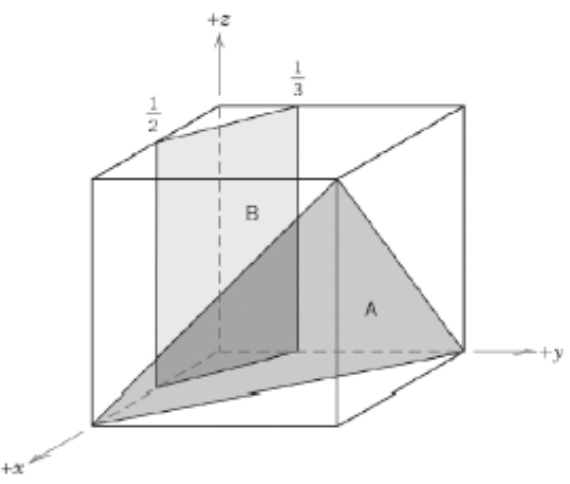
\includegraphics[width=0.5\linewidth]{../figures/e3_2.png}
  \label{fig:e3_2}
\end{figure}
\bigbreak
For A, the intercepts with the axes are $A = a$, $B = b$ and $C = -c$. We can now find the reciprocals of these as
\begin{align*}
  \frac{1}{A} &= \frac{1}{a} \\
  \frac{1}{B} &= \frac{1}{b} \\
  \frac{1}{C} &= - \frac{1}{c}
.\end{align*}
We can normalize these as 1 1 -1, which means the Miller indices become $(1 1 \overline{1})$
\bigbreak
For $B$, the intercepts with the axes are $A = \frac{1}{2}a$, $B = \frac{1}{3}b$ and $C = \infty c$. The reciprocals are thus
\begin{align*}
  \frac{1}{A} &= \frac{2}{a} \\
  \frac{1}{B} &= \frac{3}{b} \\
  \frac{1}{C} &= \frac{1}{\infty} c
.\end{align*}
These can  be normalized as 2 3 0, which means the miller indices become (230).
